\documentclass[11pt,notes=hide,aspectratio=169,mathserif]{beamer}

% ================= PREAMBLE (matches your style) =================
\usepackage{graphics}
\usepackage{graphicx}
\usepackage{url}
%\usepackage{natbib}
\usepackage{bibentry}
\usepackage{verbatim}
\usepackage{booktabs}
\usepackage{etoolbox}
\usepackage{datetime}
\usepackage{bm}
\usepackage{subcaption}
\usepackage{amsfonts}
\usepackage{amsmath}
\usepackage{amsthm}

\def\newblock{}
\linespread{1.2}

\title[class]{ECON 340: Economics of the Family \\ TA Session 5}
\author[Vaidehi's class]{Vaidehi Parameswaran (Northwestern Economics)}
\date{\monthname[\the\month] \the\year}

\usetheme{metropolis}
\definecolor{mycolor}{RGB}{48,7,144}
\setbeamercolor{frametitle}{bg=mycolor, fg=white}
\setbeamercolor{title separator}{fg=mycolor}
\setbeamercolor{progress bar}{fg=mycolor}
\beamertemplatenavigationsymbolsempty
\setbeamertemplate{footline}[frame number]{}
\setbeamertemplate{itemize item}{\small\raisebox{1pt}{\textcolor{mycolor}{$\blacktriangleright$}}}
\setbeamertemplate{itemize subitem}{\footnotesize\raisebox{1pt}{\textcolor{mycolor}{$\triangleright$}}}
\setbeamertemplate{itemize subsubitem}{\tiny\raisebox{1pt}{\textcolor{mycolor}{$\triangleright$}}}

\usepackage{hyperref}
\hypersetup{
  colorlinks=true,
  linkcolor=mycolor,
  urlcolor=mycolor,
  citecolor=mycolor
}

\usepackage{appendixnumberbeamer}
\setbeamertemplate{section in toc}{%
  \leavevmode\llap{\textcolor{mycolor}{$\blacktriangleright$}\hspace{0.6ex}}%
  \inserttocsection\par}
\setbeamertemplate{subsection in toc}{%
  \leavevmode\llap{\textcolor{mycolor}{$\triangleright$}\hspace{1.1ex}}%
  \inserttocsubsection\par}

\AtBeginSection[]{
  \begin{frame}{Today}
    \tableofcontents[currentsection]
  \end{frame}
}

\begin{document}

% ---------------------------------------------------------------
\begin{frame}[plain]
\titlepage
\end{frame}
% ---------------------------------------------------------------

\section{Can Women Have Children and a Career? (AER 2017)}



% ---------------------------------------------------------------
\begin{frame}{Motivation}
\begin{itemize}
  \item The child penalty: A key component of gender inequality
  \item In almost all labor markets, women with children work and earn less than women
  without children
  \item Estimating the causal impact of children is hard. Why?
    \pause \begin{itemize}
      \item Fertility choices are endogenous
    \end{itemize}
  \item  Causation: having children has
  adverse labor market consequences for women
  \item Adverse
  selection: women with children work and earn less, regardless of having
  children
\end{itemize}
\end{frame}
% ---------------------------------------------------------------

% ---------------------------------------------------------------
\begin{frame}{Motivation}
\begin{itemize}
  \item  Identifying the labor market effects of
  having children (the extensive fertility margin), as opposed to the labor market
  effects of having additional children among women who already have children (the
  intensive fertility margin), is very difficult
  \item Why does this matter? Most family policies (e.g., parental leave, childcare subsidies) are intended to support women with children 
  \item But the effect of these policies may be different if the selection is adverse 
\end{itemize}
\end{frame}
% ---------------------------------------------------------------

% ---------------------------------------------------------------
\begin{frame}{Today's Paper}
\small
\textbf{Lundborg, Plug \& Rasmussen (2017).} \emph{Can Women Have Children and a Career? IV Evidence from IVF Treatments.} \textit{American Economic Review}, 107(6):1611–37. \\[0.6em]
\begin{itemize}
  \item \textbf{Question:} What is the \emph{causal} effect of having (a first) child on women’s earnings and careers?
  \item \textbf{Approach:} Use \textbf{IVF treatment success at first treatment} as an instrument for fertility among \emph{childless} women in Denmark.
  \item \textbf{Why new?} Identifies effects at the \textbf{extensive margin} (becoming a mother) rather than adding an extra child.
\end{itemize}
\end{frame}
% ---------------------------------------------------------------

% ---------------------------------------------------------------
\begin{frame}{Literature Before This}
\begin{itemize}
  \item Twins at first birth (Rosenzweig and Wolpin 1980; Jacobsen, Pearce, and Rosenbloom 1999; and Vere 2011)
  \begin{itemize}
    \item Mothers with twins work less than mothers with singletons, but eventually catch up
  \end{itemize}
  \item Sex composition of first two children with preferences for mixed gender composition (Angrist and Evans 1998; Iacovou 2001; Cruces and Galiani 2007)
  \begin{itemize}
    \item Mothers with two kids of the same sex work less, because they are likely to have a third child
  \end{itemize}
  \item Useful experiments but only identify the intensive margin (additional child)
  \item But theoretically, the extensive margin is more important
\end{itemize}
\end{frame}
% ---------------------------------------------------------------

% ---------------------------------------------------------------
\begin{frame}{Setting \& Data}
\small
\begin{itemize}
  \item \textbf{Denmark:} Generous paid leave, subsidized childcare, job protections
  \item Parental leave compensation 70 - 90\% of previous earnings for up to 32 weeks 
  \item \textbf{IVF register:}  Information on all IVF treatments taking place in public and private fertility clinics in Denmark.
  \item Mandatory reporting since 1994 up to 2005
  \item Highly detailed information about the causes of infertility, number of eggs collected, and treatment outcomes (pregnancy and live birth)
  \item Linked to labor market registers, \textbf{31,666} women and \textbf{96,807} IVF treatments (1991–2009)
\end{itemize}
\end{frame}
% ---------------------------------------------------------------

% ---------------------------------------------------------------
\begin{frame}{IVF Treatment}
\small
\begin{itemize}
  \item IVF is a medical procedure to help infertile couples conceive: last resort typically 
  \item Danish National Health Care System entitles women with a referral to have three IVF treatments at no cost
  \item IVF treatment can fail at any stage of its 4-step process 
\end{itemize}
\end{frame}
% ---------------------------------------------------------------

% ---------------------------------------------------------------
\begin{frame}{IVF Treatment}
\begin{figure}
\centering
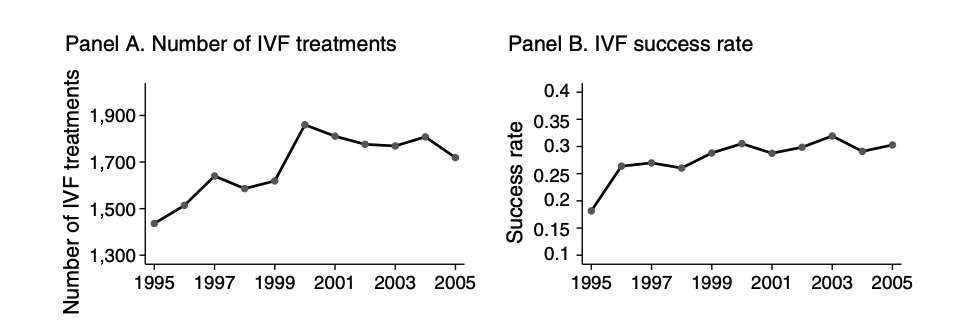
\includegraphics[width=1.0\linewidth]{inputs/ivf1.png}
\end{figure}
\begin{itemize}
  \item IVF usage increased until the year
  2000, after which usage more or less stabilized.
  \item  The IVF success rate per
  treatment increased substantially
  \end{itemize}
\end{frame}
% ---------------------------------------------------------------

% ---------------------------------------------------------------
\begin{frame}{Constructing the Instrument}
\small
\begin{itemize}
  \item The Goal: exogenous shock in IVF-driven fertility
  \item Women can undergo multiple treatments - endogenous
  \begin{itemize}
\item Restrict to first IVF treatment
  \end{itemize}
  \item Extensive margin decision 
  \begin{itemize}
    \item Focus on childless women
  \end{itemize}
  \item Want the women to be as similar as possible
  \begin{itemize}
    \item Focus on women who have successfully reached the fourth stage and had embryos implanted
  \end{itemize}
\end{itemize}
\end{frame}
% ---------------------------------------------------------------

% ---------------------------------------------------------------
\begin{frame}{Descriptive Stats}
  \begin{figure}
    \centering
    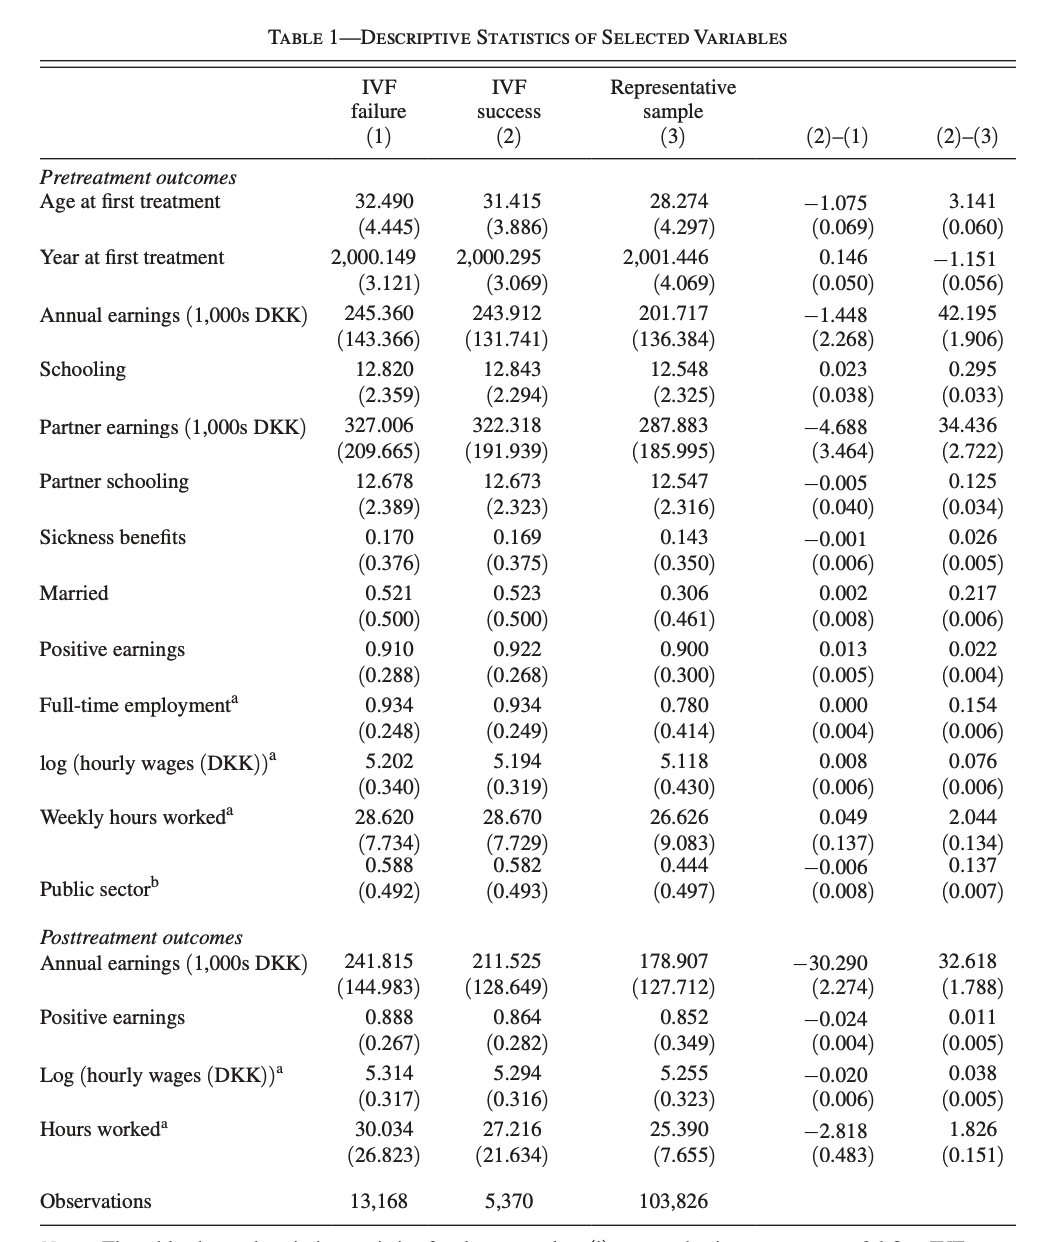
\includegraphics[width=0.8\linewidth]{inputs/ivf2.png}
    \end{figure}
\end{frame}
% ---------------------------------------------------------------
% ---------------------------------------------------------------
\begin{frame}{Descriptive Stats}
  \begin{figure}
    \centering
    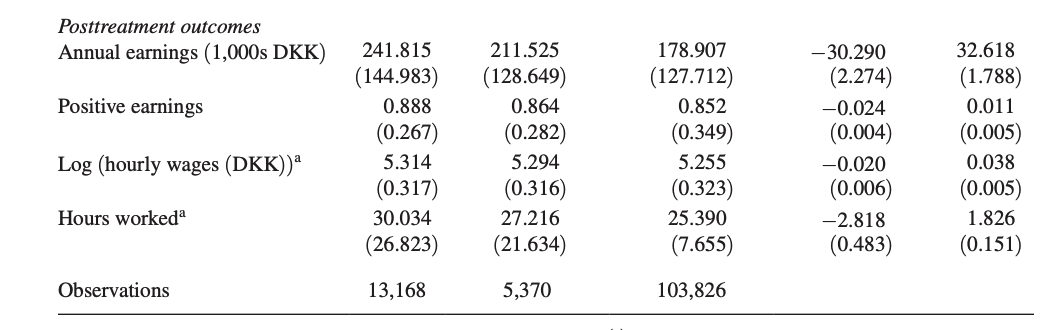
\includegraphics[width=0.8\linewidth]{inputs/ivf3.png}
    \end{figure}
\end{frame}
% ---------------------------------------------------------------


\section{IV Interlude}

% ---------------------------------------------------------------
\begin{frame}{IV Methodology}
\begin{itemize}
  \item What is an instrument? 
  \begin{itemize}
    \item Something that shifts our endogenous variable but does not directly affect our outcome variable
  \end{itemize}
  \item Two key requirements:
  \begin{itemize}
    \item Relevance: instrument must be correlated with the endogenous regressor
    \item Exogeneity: instrument must not be correlated with the error term in the outcome equation
    \end{itemize}
  \item In this setting, something that affects fertility but does not directly affect earnings or careers of women 
\end{itemize}
\end{frame}
% ---------------------------------------------------------------

% ---------------------------------------------------------------
\begin{frame}{IV 2SLS}
\begin{itemize}
  \item Structural equation:
  \[
Y_{it} = \gamma_t X_i + \delta_t F_{it} + \nu_{it}
\]
  \item First-stage equation:
  \[
F_{it} =\alpha_t X_i + \beta_t Z_i + u_{it}
\]
\item Reduced-form equation:
\[
Y_{it} = \sigma_t X_i + \pi_t Z_{it} + \nu_{it}
\]
\item Wald estimator: \(\delta_t = \frac{\pi_t}{\beta_t}\)
\end{itemize}
\end{frame}
% ---------------------------------------------------------------

% ---------------------------------------------------------------
\begin{frame}{IVF as IV}
  $\delta_t$ is identified if:
\begin{itemize}
  \item Relevance: treatment success is correlated with fertility 
  \item Exclusion: treatment success exclusively affects labor earnings through its first-stage impact on fertility
\end{itemize}
\end{frame}
% ---------------------------------------------------------------

% ---------------------------------------------------------------
\begin{frame}{IVF as IV: First-Stage}
\begin{figure}
\centering
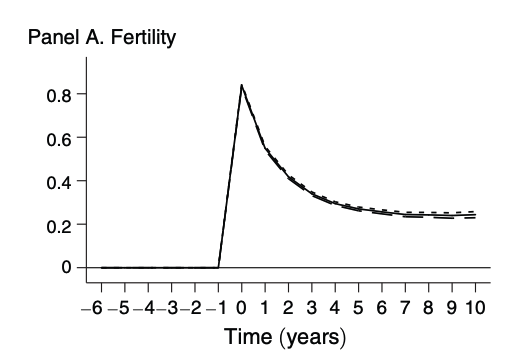
\includegraphics[width=0.6\linewidth]{inputs/ivf4.png}
\end{figure}
IVF success is strongly correlated with fertility
\end{frame}
% ---------------------------------------------------------------

% ---------------------------------------------------------------
\begin{frame}{IVF as IV: Reduced Form}
\begin{figure}
\centering
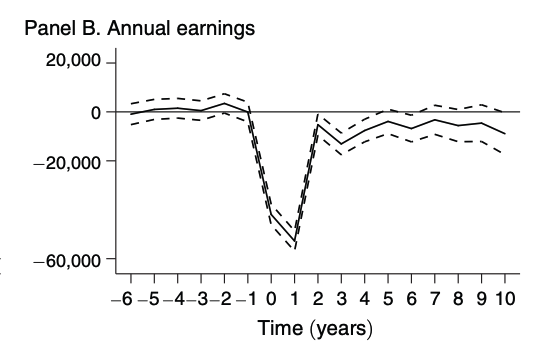
\includegraphics[width=0.6\linewidth]{inputs/ivf5.png}
\end{figure}
Women earn persistently less because
of childbearing 
\end{frame}
% ---------------------------------------------------------------

% ---------------------------------------------------------------
\begin{frame}{IVF as IV: Hours Worked}
\begin{figure}
\centering
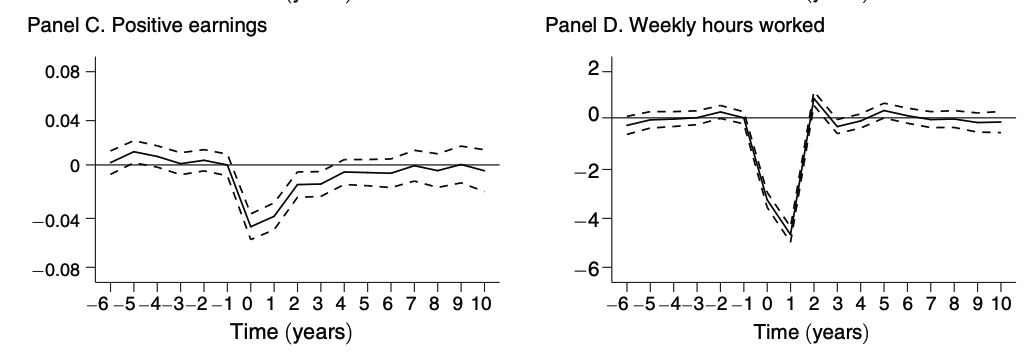
\includegraphics[width=1.0\linewidth]{inputs/ivf6.png}
\end{figure}
Women work less immediately after but eventually return
\end{frame}
% ---------------------------------------------------------------

% ---------------------------------------------------------------
\begin{frame}{IVF as IV: Hourly Wages}
\begin{figure}
\centering
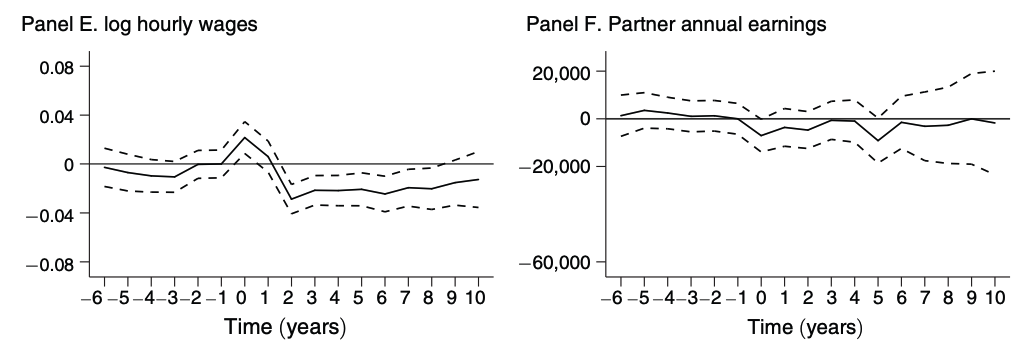
\includegraphics[width=1.0\linewidth]{inputs/ivf7.png}
\end{figure}
No effect in first two years but persistent wage penalty thereafter; no effects on partner's earnings
\end{frame}
% ---------------------------------------------------------------

% ---------------------------------------------------------------
\begin{frame}{IVF as IV: Ruling Out Other Channels}
\begin{figure}
\centering
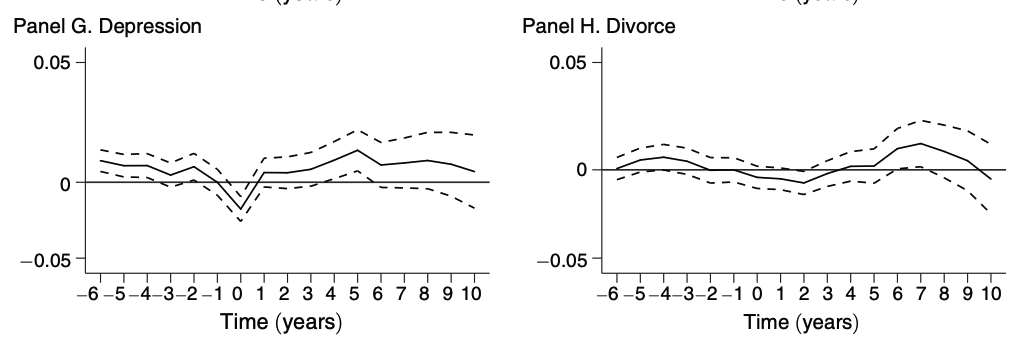
\includegraphics[width=1.0\linewidth]{inputs/ivf8.png}
\end{figure}
Little evidence of either divorce or depression effects
\end{frame}
% ---------------------------------------------------------------

% ---------------------------------------------------------------
\begin{frame}{IV Estimation}
\begin{figure}
\centering
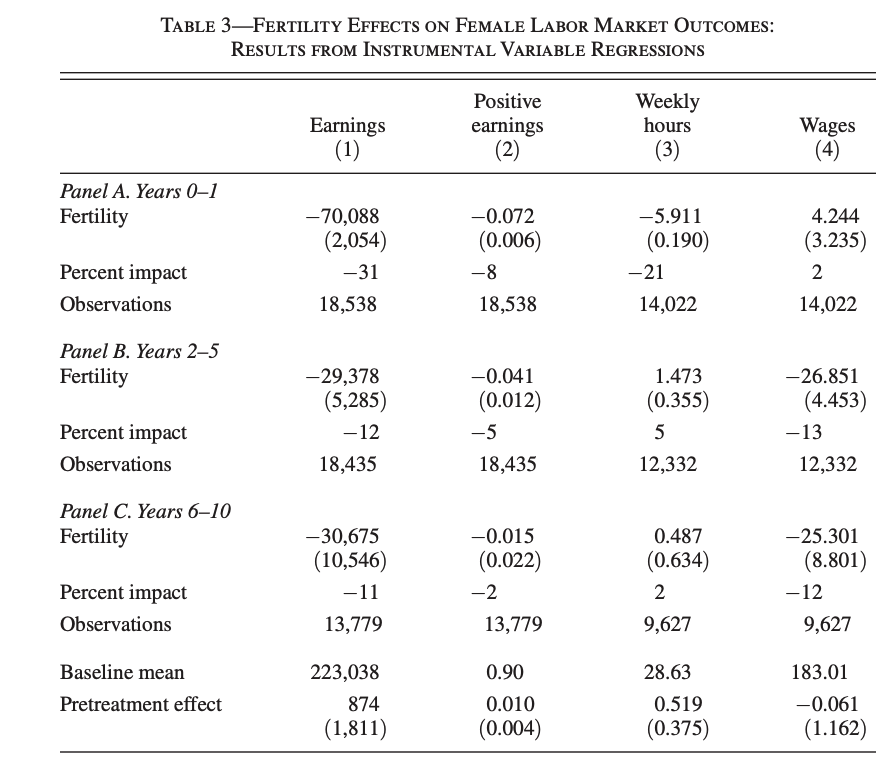
\includegraphics[width=0.5\linewidth]{inputs/ivf9.png}
\end{figure}
Having children reduces earnings by DKK 70,000 in the short run, DKK 30,000 in the medium run, and DKK 30,000 in the long run
\end{frame}
% ---------------------------------------------------------------

% ---------------------------------------------------------------
\begin{frame}{IV Estimation}
\begin{figure}
\centering
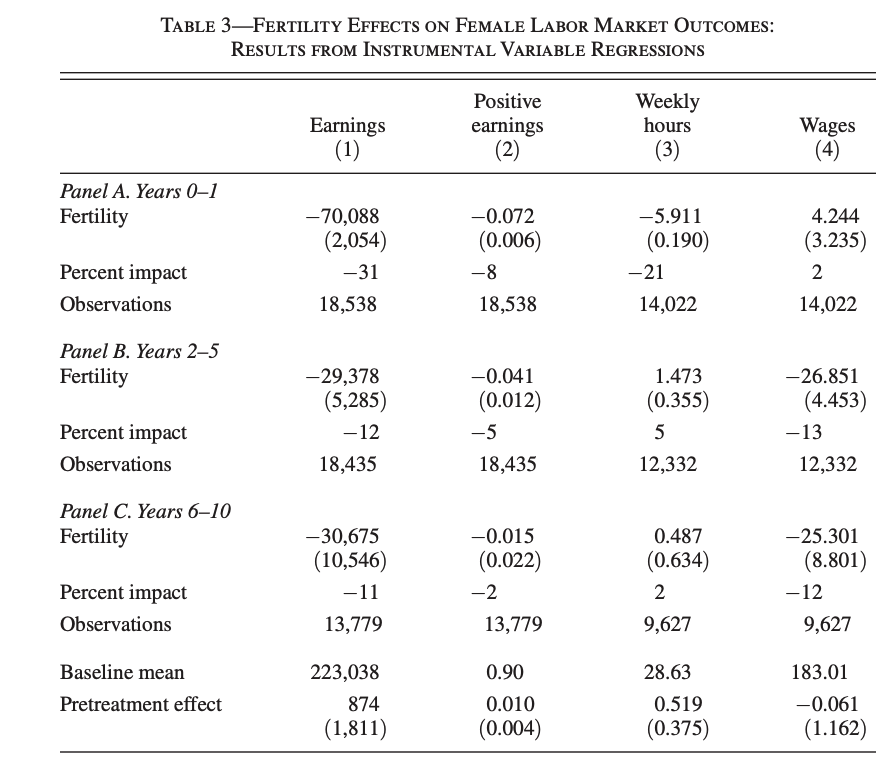
\includegraphics[width=0.5\linewidth]{inputs/ivf9.png}
\end{figure}
Women work less because of children, but only when children are young \\
Significant, negative, and large effects in the medium and long run
\end{frame}
% ---------------------------------------------------------------

% ---------------------------------------------------------------
\begin{frame}{Why do women earn less?}
\pause \begin{figure}
\centering
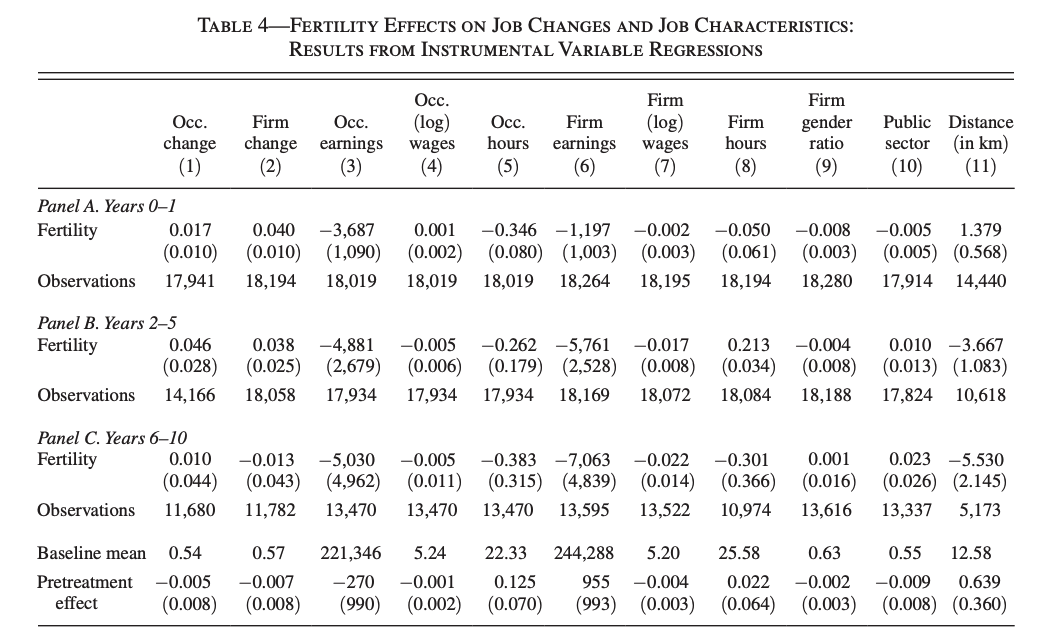
\includegraphics[width=0.9\linewidth]{inputs/ivf10.png}
\end{figure}
\end{frame}
% ---------------------------------------------------------------



% ---------------------------------------------------------------
\begin{frame}{Job Moves \& Commuting Distance}
\begin{itemize}
  \item Mothers more likely to \textbf{change occupation/firm} in 0–5 years.
  \item By 6–10 years, women with children work \textbf{closer to home}: long-run commute distance 5.5 km lower
  \item Suggestive of job re-sorting toward proximity/flexibility; small declines in average occupation and firm earnings premia.
\end{itemize}
\end{frame}
% ---------------------------------------------------------------

% ---------------------------------------------------------------
\begin{frame}{Heterogeneity}
  \begin{figure}
    \centering
    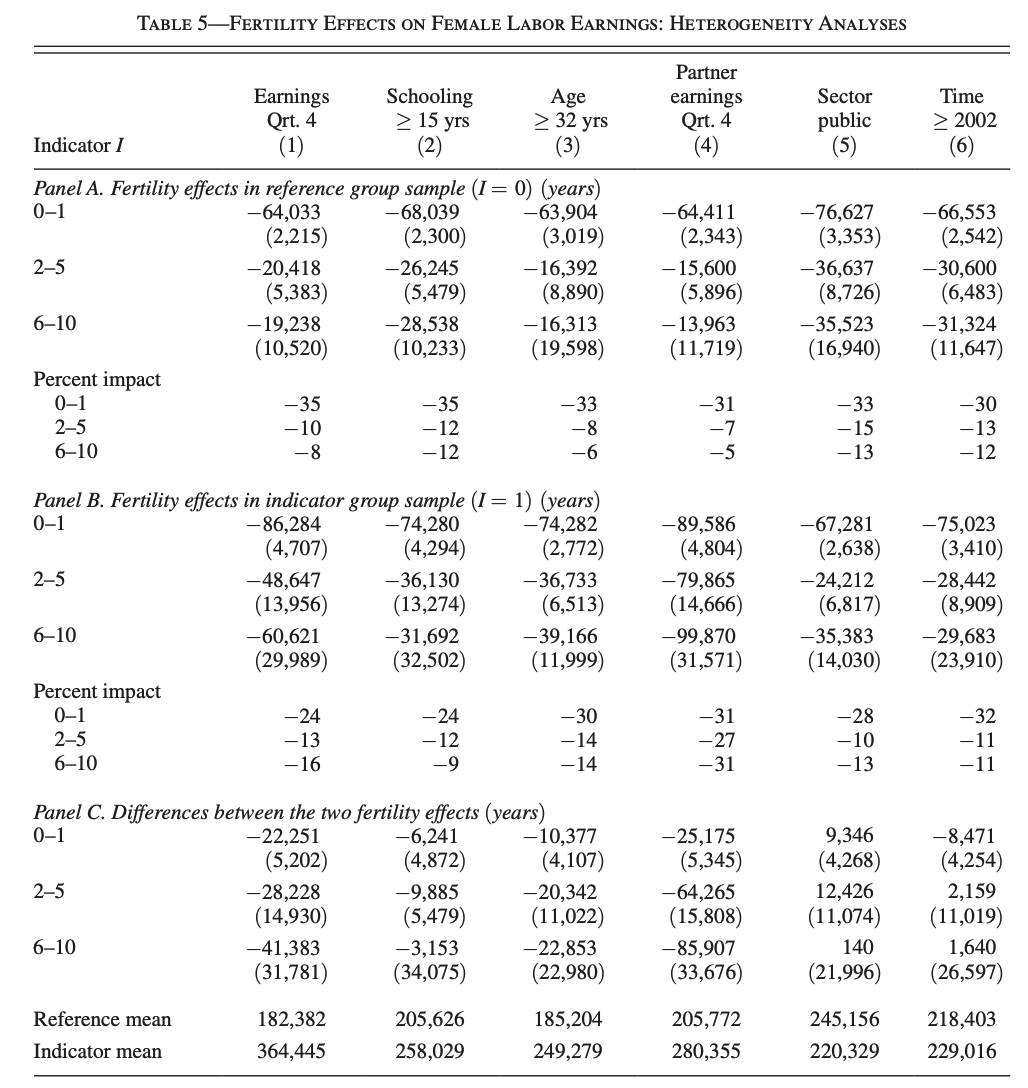
\includegraphics[width=0.9\linewidth]{inputs/ivf11.png}
    \end{figure}
    Partner's earnings are most important
\end{frame}
  % ---------------------------------------------------------------



% ---------------------------------------------------------------
\begin{frame}{Extensive vs. Intensive Margin}
\small
\begin{itemize}
  \item Compare childless women to women who already have children at the start of IVF treatment
  \item Also exploit the larger prevalence of twins among IVF births
\end{itemize}
\end{frame}
% ---------------------------------------------------------------

% ---------------------------------------------------------------
\begin{frame}{Extensive vs. Intensive Margin}
  \begin{figure}
    \centering
    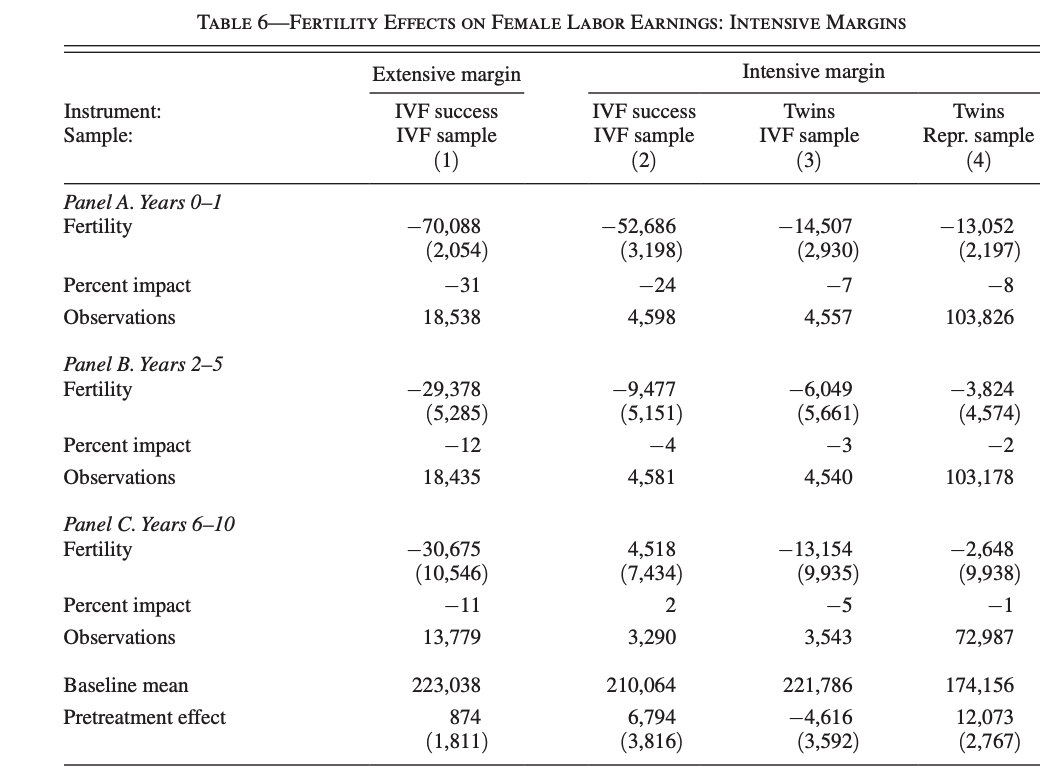
\includegraphics[width=0.6\linewidth]{inputs/ivf12.png}
    \end{figure}
    Measured at the intensive margin, effects are relatively small and mostly short lived
  \end{frame}
  % ---------------------------------------------------------------

% ---------------------------------------------------------------
\begin{frame}{Conclusion}
\small
\begin{itemize}
  \item Short run: \textbf{leave/participation/hours} drive initial loss.
  \item Medium/long run: \textbf{wage penalties} persist via job re-sorting (closer to home; slightly lower-paying occupation/firm averages).
  \item Consistent with career track interruptions, reduced accumulation of specific human capital, and job mobility toward family-friendly matches.
  \item Are these results generalizable? In settings with less generous benefits and support? 
\end{itemize}
\end{frame}
% ---------------------------------------------------------------


%---------------------------------------------------------------------
\begin{frame}
\begin{center}{\LARGE See you next time!}\end{center}
\end{frame}
%---------------------------------------------------------------------

\end{document}
